
\documentclass{beamer} 


\mode<presentation>
{
  \usetheme{Berkeley}
  % or ...

  \setbeamercovered{transparent}
  % or whatever (possibly just delete it)
}

\usepackage{tikz}
\usepackage{graphicx}
\usepackage[english]{babel}
\usepackage{wrapfig}
% or whatever

\usepackage[utf8]{inputenc}
% or whatever

\usepackage{times}
\usepackage[T1]{fontenc}
% Or whatever. Note that the encoding and the font should match. If T1
% does not look nice, try deleting the line with the fontenc.


\title[Next Steps in Research Transparency] % (optional, use only with long paper titles)
{Next Steps in Research Transparency}

\subtitle
{Where do we go from here?}

\author[Christensen] % (optional, use only with lots of authors)
{Garret~Christensen\inst{1}}
% - Give the names in the same order as the appear in the paper.
% - Use the \inst{?} command only if the authors have different
%   affiliation.

\institute[University of California Berkeley] % (optional, but mostly needed)
{
  \inst{1}%
  Berkeley Initiative for Transparency in the Social Sciences\\
  UC Berkeley
  }
% - Use the \inst command only if there are several affiliations.
% - Keep it simple, no one is interested in your street address.

\date[BITSS2015] % (optional, should be abbreviation of conference name)
{BITSS Summer Institute 2015}
% - Either use conference name or its abbreviation.
% - Not really informative to the audience, more for people (including
%   yourself) who are reading the slides online

\subject{Research Transparency}
% This is only inserted into the PDF information catalog. Can be left
% out. 



% If you have a file called "university-logo-filename.xxx", where xxx
% is a graphic format that can be processed by latex or pdflatex,
% resp., then you can add a logo as follows:

 \pgfdeclareimage[height=2cm]{university-logo}{BITSSlogo.png}
 \logo{\pgfuseimage{university-logo}}



% Delete this, if you do not want the table of contents to pop up at
% the beginning of each subsection:
%\AtBeginSubsection[]
%{
%  \begin{frame}<beamer>{Outline}
%    \tableofcontents[currentsection,currentsubsection]
%  \end{frame}
%}


% If you wish to uncover everything in a step-wise fashion, uncomment
% the following command: 

%\beamerdefaultoverlayspecification{<+->}


\begin{document}

\begin{frame}
  \titlepage
\end{frame}

%%%%%%%%%%%%%%%%%%%%%%%%%%%%%%%%%%%%%%%%%%%%%%%%%%%%%%%%%%%%%%%%%%%%%%
\begin{frame}{Outline}
\tableofcontents
\end{frame}
%%%%%%%%%%%%%%%%%%%%%%%%%%%%%%%%%%%%%%%%%%%%%%%%%%%%%%%%%%%%%%%%%%%%%%
\section{BITSS Activities}

\subsection{Manual of Best Practices}
 \begin{frame}{Manual of Best Practices}
 Our goal:
 \begin{itemize}
 \item
 Detailed hands-on how-to manual for transparent social science research. 
 \item 
 Cover all aspects of a transparent research project, from beginning (study design, hypothesis registration) to end (publication, data sharing).
 \item 
 Keep the manual updated.
 \item
 Encourage participation from the community. \url{http://github.com/garretchristensen}
 \item 
 Extend into short textbook.
 \end{itemize}
\end{frame} 
%%%%%%%%%%%%%%%%%%%%%%%%%%%%%%%%%%%%%%%%%%%%%%%%%%%%%%%%%%%%%%%%%%%%%
%%%%%%%%%%%%%%%%%%%%%%%%%%%%%%%%%%%%%%%%%%%%%%%%%%%%%%%%%%%%%%%%%%%%%%%%%
\subsubsection*{Ethical Research}
\begin{frame}{Ethical Research}
\begin{itemize}
\item
Transparency is part of being an ethical researcher. 
\item
Fraud exists (Simonsohn 2013), but mostly we should admit that we're human, subject to bias and motivated reasoning, transparency can help with this (Nosek, Spies, Motyl 2012).
\item
Since a lot of us run experiments, we should take IRBs seriously as part of transparency (Ch. 11--13 Morton \& Williams 2010, Desposato 2014). 
\end{itemize}
\end{frame}

%%%%%%%%%%%%%%%%%%%%%%%%%%%%%%%%%%%%%%%%%%%%%%%%%%%%%%%%%%%%%%%%%%
\subsubsection*{Study Design and Power}
\begin{frame}{Study Design and Power}
\begin{itemize}[<.->]
\item
Adequately power trials to help prevent spurious significant results. 
\item
Practical suggestions:
\begin{itemize}
\item
Collaborate with other labs to mutually run each others' experiments (Open Science Collaboration 2014).
\item
Maximize power subject to budget constraint by adjusting expensive treatment arm (relative) size (Duflo, Glennerster, Kremer 2007). 
\end{itemize}
\end{itemize}
\end{frame}

%%%%%%%%%%%%%%%%%%%%%%%%%%%%%%%%%%%%%%%%%%%%%%%%%%%%%%%%%%%%%%%%%%%%%
\subsubsection*{Publication Bias}
\begin{frame}{Publication Bias}%{Subtitles are optional.}
  % - A title should summarize the slide in an understandable fashion
  %   for anyone how does not follow everything on the slide itself.
  Existence of the problem:
  \begin{itemize}[<.->]
  \item
 Effect sizes diminish with sample size (Gerber, Green, Nickerson 2001)
  \item
  There is a higher fraction of rejected hypothesis tests in social compared to hard sciences (Fanelli 2010).
  \item
  	Published null results are disappearing over time, in all disciplines (Fanelli 2011). 
  \item
  	Data on the complete set of experiments run shows strong results are 40pp more likely to be published, and 60pp more likely to be written up. The file drawer problem is large. (Franco, Malhotra, Simonovits 2014)
  	\item
  	If we only write up/publish significant results, and we have no record of all the insignificant results, we have no way to tell if our `significant' results are real, or if they're the 5\% we should expect due to noise.
  \end{itemize}
\end{frame}

%{ % all template changes are local to this group.
%    \setbeamertemplate{navigation symbols}{}
%    \begin{frame}[plain]
%        \begin{tikzpicture}[remember picture,overlay]
%            \node[at=(current page.center)] {
%                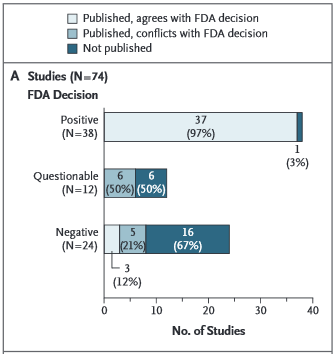
\includegraphics[height=\paperheight]{TurnerFigure1.PNG}
%            };
%        \end{tikzpicture}
%     \end{frame}
%}

%\begin {frame}{Publication Bias}
%\end{frame}

\subsubsection*{Registrations}
\begin{frame}{Registration}
Registration as Solution to Publication Bias:
 \begin{itemize}
  \item
   Publicly stating all research you will do, what hypotheses you will test, prospectively.
   %\item If we know every hypothesis test that is run on a given subject, we have a better idea of how seriously to take the significant results.
  \item
   Near universal adoption in medical RCTs. Top journals (ICMJE) won't publish if it's not registered. \url{http://clinicaltrials.gov}
  \item
   Even better if registry requires outcomes from after study. Currently limited, but NIH is moving on this.
   \item Newer to social sciences, but:
   \begin{itemize}[<.->]
   \item
   	AEA registry, currently only for RCTs. \url{http://socialscienceregistry.org}
   \item
    EGAP registry \url{http://egap.org/design-registration}
   \item 
    3ie registry, for developing country evaluations. \url{http://ridie.3ieimpact.org}
   \item
   	Open Science Framework\\ \url{http://osf.io}
   \end{itemize}
  \end{itemize}  
\end{frame}


%%%%%%%%%%%%%%%%%%%%%%%%%%%%%%%%%%%%%%%%%%%%%%%%%%%%%%%%%%%%%%
\begin{frame}{Meta-Analysis}
\begin{itemize}
\item Synthesize results systematically
\item Cochrance Collaboration (medicine), Campbell Collaboration (policy), What Works Clearinghouse
\item Funnel plots (Card \& Krueger 1995)
\item P-curve (Simonsohn et al. 2014)
\end{itemize}
\end{frame}
%%%%%%%%%%%%%%%%%%%%%%%%%%%%%%%%%%%%%%%%%%%%%%%%%%%%%%%%%%%%%%%%%%%%%%%
\subsubsection*{P-Hacking}
\begin{frame}[<.->]{P-Hacking}
Define the problem:
\begin{itemize}
\item
Also called fishing, researcher degrees of freedom, or data-mining.
\item
Definition: flexibility in data analysis allows portrayal of \textit{anything} as below an arbitrary p-value threshhold; significance loses its meaning.
\item
Not something only evil people do. It's subconcious, or simply built into statistics (Gelman, Loken 2013).
\end{itemize}
\end{frame}

\subsubsection*{Pre-Analysis Plan}
\begin{frame}{Pre-Analysis Plan}
Explain the solution:
\begin{itemize}
\item
From 3ie: ``A pre-analysis plan is a detailed description of the analysis to be conducted that is written in advance of seeing the data on impacts of the program being evaluated. It may specify hypotheses to be tested, variable construction, equations to be estimated, controls to be used, and other aspects of the analysis. A key function of the pre-analysis plan is to increase transparency in the research. By setting out the details in advance of what will be done and before knowing the results, the plan guards against data mining and specification searching. Researchers are encouraged to develop and upload such a plan with their study registration, but it is not required for registration.''
\end{itemize}
\end{frame}

%\begin{frame}{Origin: FDA's Guidance for Industry}
%``E9 Statistical Principles for Clinical Trials'' (1998)
%\href{http://www.fda.gov/downloads/drugs/guidancecomplianceregulatoryinformation/guidances/ucm073137.pdf}{\beamergotobutton{Link}}
%\S V Data Analysis Considerations
%\begin{enumerate}
%\item Prespecification of the Analysis
%\item Analysis Sets
%\item Missing Values and Outliers
%\item Data Transformation
%\item Estimation, Confidence Intervals, and Hypothesis Testing
%\item Adjustment of Significance and Confidence Levels
%\item Subgroups, Interactions, and Covariates
%\item Integrity of Data and Computer Software Validity
%\end{enumerate}
%\end{frame}


%\begin{frame}{Glennerster, Takavarasha Suggestions}
%\textit{Running Randomized Evaluations}
%\begin{enumerate}[<.->]
%\def\labelenumi{\arabic{enumi}.}
%\item
%  the main outcome measures,
%\item
%  which outcome measures are primary and which are secondary,
%\item
%  the precise composition of any families that will be used for mean effects analysis,
%  \begin{itemize}
%  \item Explain mean effects, FWER, FDR using Anderson (JASA 2008).
%  \end{itemize}
%\item
%  the subgroups that will be analyzed,
%\item
% the direction of expected impact if we want to use a one-sided test, and
%\item the primary specification to be used for the analysis.
%\end{enumerate}
%\end{frame}

%\begin{frame}{McKenzie Suggestions}
%\href{http://blogs.worldbank.org/impactevaluations/a-pre-analysis-plan-checklist}{World Bank Development Impact Blog}

%\begin{enumerate}[<.->]
%\item
%  Description of the sample to be used in the study
%\item  Key data sources
%\item Hypotheses to be tested throughout the causal chain
%\item
%  Specify how variables will be constructed
%\item  Specify the treatment effect equation to be estimated
%\item  What is the plan for how to deal with multiple outcomes and multiple
%  hypothesis testing?
%\item  Procedures to be used for addressing survey attrition
%\item  How will the study deal with outcomes with limited variation?
%\item  If you are going to be testing a model, include the model
%\item  Remember to archive it
%\end{enumerate}
%\end{frame}

%\begin{frame}{Examples}
%\begin{itemize}[<.->]
%\item J-PAL Hypothesis Registry (11), see \url{http://www.povertyactionlab.org/Hypothesis-Registry}

%6 published papers:
%\begin{itemize}
%\item Sierra Leone CDD, Oregon Medicare, Turkey Job Training, El Salvador TOMS, two in Indonesia (Olken et al.)
%\end{itemize}
%\item Psychology: \href{http://pss.sagepub.com/content/26/2/249}{Hawkins, Fitzgerald, Nosek---Conception Risk and Prejudice}
%\end{itemize} 
%\vspace{0.25in}
%Wide range of when exactly to write and how detailed to make the plan. At the extreme level of detail you would have your entire code already written before you got any data.
%\end{frame}

%%%%%%%%%%%%%%%%%%%%%%%%%%%%%%%%%%%%%%%%%%%%%%%%%%%%%%%%%%%%%%%%%%%%
\subsubsection*{Replication}
\begin{frame}{Replication}
\begin{enumerate}[<.->]
 \item The Problem	(JMCB Project)
 \item Project Protocol, Reporting Standards
 \item Organizing Workflow
 \item Code \& Data Sharing
\end{enumerate}
\end{frame}

\subsubsection*{Project Protocol, Reporting Standards}
\begin{frame}[<.->]{Project Protocol, Reporting Standards}
 Make sure you report everything another researcher would need to replicate your research.
 \begin{itemize}
 \item Find the appropriate reporting standard for your field and follow it: \url{http://www.equator-network.org/}
\item Report the nuts and bolts of the project implementation in a detailed protocol: \url{http://www.spirit-statement.org}
\end{itemize}
\end{frame}

 \subsubsection*{Workflow}
 \begin{frame}{Workflow}
``Reproducibility is just collaboration with people you don't know,
including yourself next week''

---Philip Stark, UC Berkeley Statistics

\vspace{0.15in}

Practical coding and organizational suggestions
 \begin{itemize}
 \item Long (2008) \textit{The Workflow of Data Analysis Using Stata}
 \begin{itemize}
 	\item Making any changes to a file that has been posted/shared means it gets a new name.
 	\item Use version commands to ensure others get same results.
  \end{itemize}
 \item Literate programming (extensive commenting, making the aim of code reading by a human)
 \item Dynamic Documents (R Markdown): integration of analysis and output.
\end{itemize}
\end{frame}

\subsubsection*{Data Sharing}
\begin{frame}{Data Sharing}
Post your code and your data in a trusted public repository.
\begin{itemize}[<.->]
\item
Find the appropriate repository: \url{http://www.re3data.org/}
\item
Repositories will last longer than your own website.
\item
Repositories are more easily searchable by other researchers.
\item
Repositories will store your data in a non-proprietary format that won't become obsolete.
\end{itemize}
\end{frame}
%%%%%%%%%%%%%%%%%%%%%%%%%%%%%%%%%%%%%%%%%%%%%%%%%%%%%%%
\subsection{Meta-Research Grant Initiative}
\begin{frame}{Meta-Research Grant Initiative}
Funding will be primarily directed to methodological research projects that advance understanding and design of new approaches for reproducibility and reliability. (\$15K-\$30K)
\begin{itemize}
\item Laura and John Arnold Foundation
\item RFP this summer!
\item Analysis of various pre-specification practices, including impacts on reported research findings;
\item Application of specification curves to existing influential studies in economics;
\item Experiments involving the research community to reveal the effects of a researchers’ degrees of freedom on study outcomes;
\item Cumulative meta-analyses, to track the evolution of a body of evidence over time;
\end{itemize}

Also, recent small grants from Sloan Foundation for data publication.

\end{frame}

%%%%%%%%%%%%%%%%%%%%%%%%%%%%%%%%%%%%%%%%%%%%%%%%%%%%%%
\subsection{Leamer-Rosenthal Prizes}
\begin{frame}{Leamer-Rosenthal Prizes}

\begin{itemize}
\item Emerging Leaders in Open Social Science Research – up to \$15,000
\href{http://www.bitss.org/prizes}{\beamerbutton{Link}}

\item 
Focusing on young scholars, this prize will reward graduate students, postdoctoral researchers, and junior faculty who have (i) authored papers demonstrating exceptionally transparent and reproducible research practices, or (ii) engaged in projects advancing our understanding of research transparency and/or methodological tools to achieve this objective.

\item Leaders in Open Social Science Education – up to \$10,000

\item This prize will reward university instructors at top-tier research institutions who have developed a curriculum on research transparency, or incorporated at least three lectures on the topic into a relevant course. 

\item Templeton Foundation
\end{itemize}
\end{frame}

%%%%%%%%%%%%%%%%%%%%%%%%%%%%%%%%%%%%%%%%%%%%%%%%%%%%%%%%%%
\subsection{Developing Country Researcher Transparency}
\begin{frame}{Open Research from Developing Countries}
Potential new initiative
\begin{itemize}
\item Incorporate transparency with CEGA, train African researchers
\item EASST Scholars
\item Hewlett Foundation
\item More developing country students here.
\end{itemize}


\end{frame}
%%%%%%%%%%%%%%%%%%%%%%%%%%%%%%%%%%%%%%%%%%%%%%%%%%%%%%%%%%%
\subsection{Help Desk}
\begin{frame}{Help Desk}
BITSS collaborates with Center for Open Science to provide free statistical/reproducibility consulting. \href{http://centerforopenscience.org/stats_consulting/}{\beamerbutton{Link}}
\begin{itemize}
\item Free one-one-one consulting
\item Workshops
\end{itemize}
\end{frame}
%%%%%%%%%%%%%%%%%%%%%%%%%%%%%%%%%%%%%%%%%%%%%%%%%%%%%%%%%%%%
\subsection{BITSS Research}
\begin{frame}{BITSS Research}
\begin{itemize}
\item Christensen, Dafoe, Miguel: Data Sharing and Citations
\item BITSS Annual Meeting (December, open call)
\item BITSS-organized session at AEA/ASSA meeting
\item APPAM, APSA, OpenCon?
\end{itemize}
\end{frame}
%%%%%%%%%%%%%%%%%%%%%%%%%%%%%%%%%%%%%%%%%%%%%%%%%%%%%%%%%%%%%%%%
\subsection{BITSS Education}
\begin{frame} {BITSS Education}
\begin{itemize}
\item Econ 270D
\item Available as Youtube Playlist \href{https://www.youtube.com/playlist?list=PL-XXv-cvA_iBN9JZND3CF91aouSHH9ksB}{\beamerbutton{Link}}
\item EdX MOOC under contstruction (BITSS/J-PAL)
\end{itemize}
\end{frame}
%%%%%%%%%%%%%%%%%%%%%%%%%%%%%%%%%%%%%%%%%%%%%%%%%%%%%%%%%%%%%%%%%%%%%%%%%%%%%%%%%%%
\section{Partner Activities}
\subsection{Center for Open Science}
\subsection{Other Orgs}
\begin{frame}{Partner Activities}
\begin{itemize}
 \item
 Center for Open Science
 \begin{itemize}
 \item OSF suggestions welcome. COS Community \href{http://centerforopenscience.org/involved_participate/}{\beamerbutton{Link}}
 \item Pre-Reg Prize (Get \$1000) \href{http://centerforopenscience.org/prereg/}{\beamerbutton{Link}}
 \item Badges
 \item Design-based Publication (Registered Reports)
 \item TOP Guidelines
 \end{itemize}
\item Berkeley Institute for Data Science (\href{http://bids.berkeley.edu}{BIDS})
\begin{itemize}
\item Also at UW, NYU.
\end{itemize}
\item Meta-Research Innovation Center at Stanford (\href{http://metrics.stanford.edu}{METRICS}) 
\item Teaching Integrity in Empirical Research (\href{http://www.haverford.edu/TIER/}{TIER})
\begin{itemize}
\item Small teaching grants, October workshop (apply now!)
\end{itemize}
\end{itemize}
\end{frame}
%%%%%%%%%%%%%%%%%%%%%%%%%%%%%%%%%%%%%%%%%%%%%%%%%%%%%%%%%%%%%%%%%%%%
\subsection{Badges}
\begin{frame}{Badges to Acknowledge Open Practices}
\begin{wrapfigure}[6]{r}[0pt]{1.5cm}

\includegraphics[width=0.9\linewidth]{data.png}


\includegraphics[width=0.9\linewidth]{materials.png}


\includegraphics[width=0.9\linewidth]{preregistered.png}
\end{wrapfigure}
3 Badges \href{https://osf.io/tvyxz/wiki/home/}{\beamerbutton{Link}}
\begin{itemize}
\item Tech based on \href{Mozilla Open Badges}{http://openbadges.org/}
\item 9+ journals
\begin{itemize}
\item Open Data
\item Open Materials
\item Preregistered
\end{itemize}
\end{itemize}

\end{frame}
%%%%%%%%%%%%%%%%%%%%%%%%%%%%%%%%%%%%%%%%%%%%%%%%%%%%%%%%%%%%%%%%%%%%
\subsection{Design-Based Publication}
\begin{frame}{Design-Based Publication}
AKA Registered Reports, moves peer review before data gathering, results, and analysis.

\begin{enumerate}[<.->]
\item Design a project
\item Submit
\item Reviewed based on importance of question and quality of design
\item Get in-principle acceptance
\item Follow through, and nulls get published
\end{enumerate}
\href{https://osf.io/8mpji/wiki/home/}{14 Journals, 4 more with Special Issues \beamergotobutton{Link}}
\end{frame}
%%%%%%%%%%%%%%%%%%%%%%%%%%%%%%%%%%%%%%%%%%%%%%%%%%%%%%%%%%%%%%%%%%%%
\subsection{Transparency \& Openness Promotion Guidelines}
\begin{frame}{Transparency \& Openness Promotion Guidelines}
\begin{itemize}
\item November 2014 COS, AAAS, BITSS Meeting

\item Guidelines for journals on citation standards, data \& code \& materials sharing, design, registration of study, pre-analysis plan, replication.

\item Forthcoming in \textit{Science} at the end of the month. 

\item 50+ journals endorsed already.
\end{itemize} 
\end{frame}
%%%%%%%%%%%%%%%%%%%%%%%%%%%%%%%%%%%%%%%%%%%%%%%%%%%%%%%%%%%%%%%%%%%%%%%%%%%%%%%%%%%
\section{You}
\begin{frame}{Your Research}
\begin{itemize}
\item Register your trial.
\item Write a PAP.
\item Write code (not Excel).
\item Literate Programming (i.e. comment the hell out of your code).
\item Use version control.
\item Write reproducible dynamic documents.
\item Share your data.
\item Submit reproducible code when you submit your paper?
\item Include meta-analysis/replication in your work.
\end{itemize}
\end{frame}

\begin{frame}{Your Participation}
\begin{itemize}
\item Last year's Summer Institute Participants
\begin{itemize}
\item Brazil: opinion piece in \textit{Revista Política Hoje}.  \href{http://bitss.org/2014/11/19/replication-brazil/}{\beamerbutton{Link}}
\item Sweden: transparency training \href{http://bitss.org/2014/10/28/swedish-graduate-student-training/}{\beamerbutton{Link}}
\item Berkeley: P-curve the What Works Clearinghouse, Clearinghouse for Labor Evaluation and Research, published observational PAP. \href{http://obsstudies.org/journal.php?id=17}{\beamerbutton{Link}}
\item Spain: Barcelona Graduate School of Economics presentatation on PAP
\end{itemize}
\item Organize a conference session?
\item Stay in touch (awais@berkeley.edu, garret@berkeley.edu). New: Jenn, Shyan.
\item Blog for us! 
\item Tweet @UCBITSS!
\end{itemize}
\end{frame}


\end{document}


